\section{Вычислительные эксперименты}
    \subsection{Модель Лотки-Вольтерры}
    Возьмём параметры для модели:
    \[
        \begin{split}
            & \xi_1 = 10, \xi_2 = 8, \xi_3 = 6, \\
            & \alpha_{12} = 6, \alpha_{13} = 2, \alpha_{23} = 0.5, \\
            & k_{12} = 4, k_{13} = 1, k_{23} = 0.5.
        \end{split}
    \]

    При этом точка равновесия \( x^{(4)} = ( -3.458\dots, 46.66\dots, -150 ) \). Откуда получаем \( b_3 = -22040 \Rightarrow \Delta_2 = 22040 > 0 \). Значит, что по какой-то оси она будет устойчивая, по второй неустойчива, а по третьей устойчивость неизвестна. Однако, вероятно, это точка не будет иметь влияния, поскольку находится на большом удалении в отрицательных координатах.

    \subsubsection{При вымершей первой популяции}

    \begin{figure}[H]
        \centering
        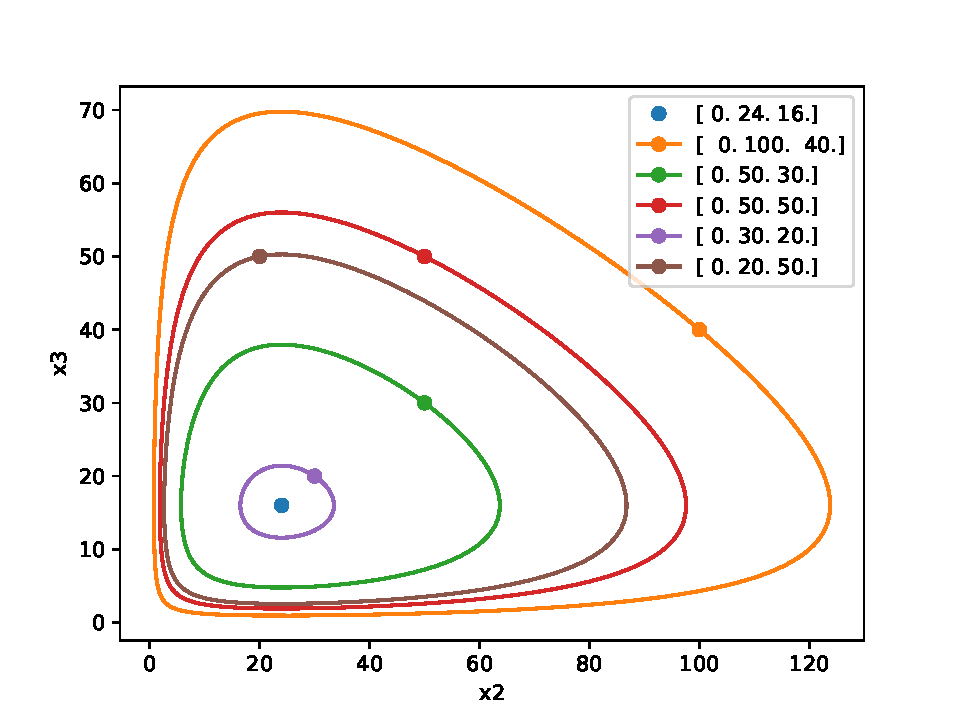
\includegraphics[width=8cm]{pictures/x1_0phase.pdf}
        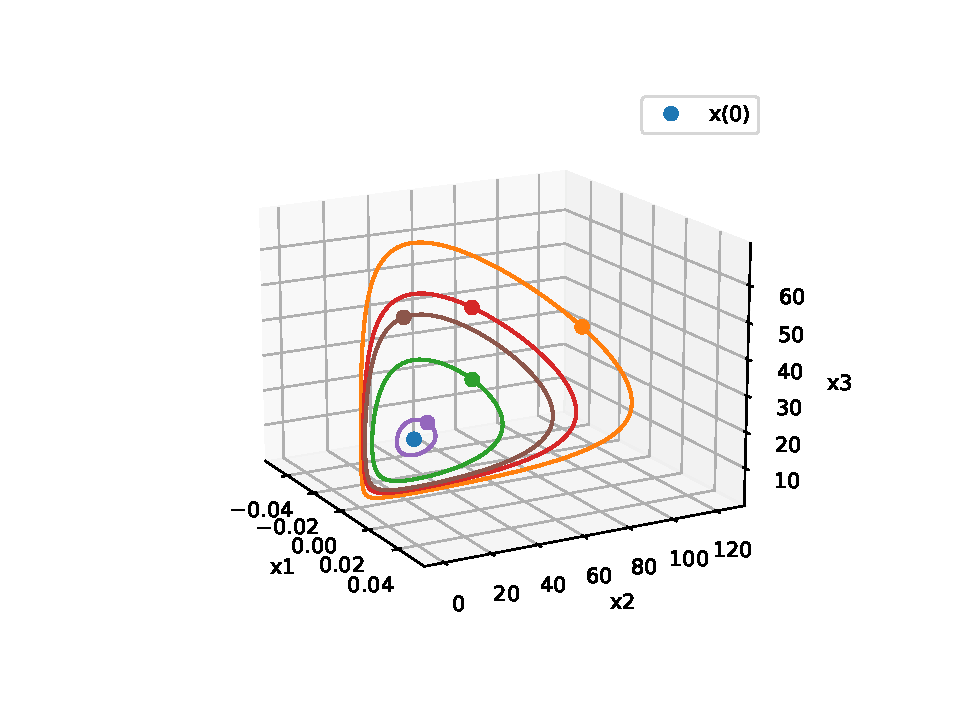
\includegraphics[width=8cm]{pictures/x1_0phase3.pdf}
        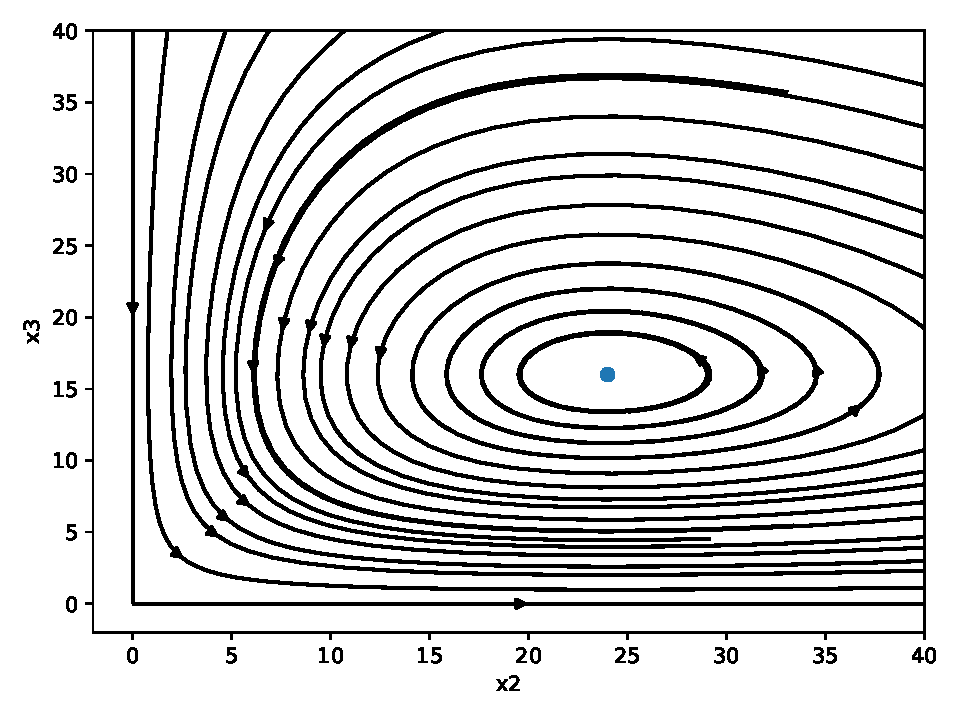
\includegraphics[width=8cm]{pictures/x1_0vector.pdf}
        \caption{На отрезке времени \( [0, 3] \).}
    \end{figure}


    \subsubsection{При вымершей второй популяции}

    \begin{figure}[H]
        \centering
        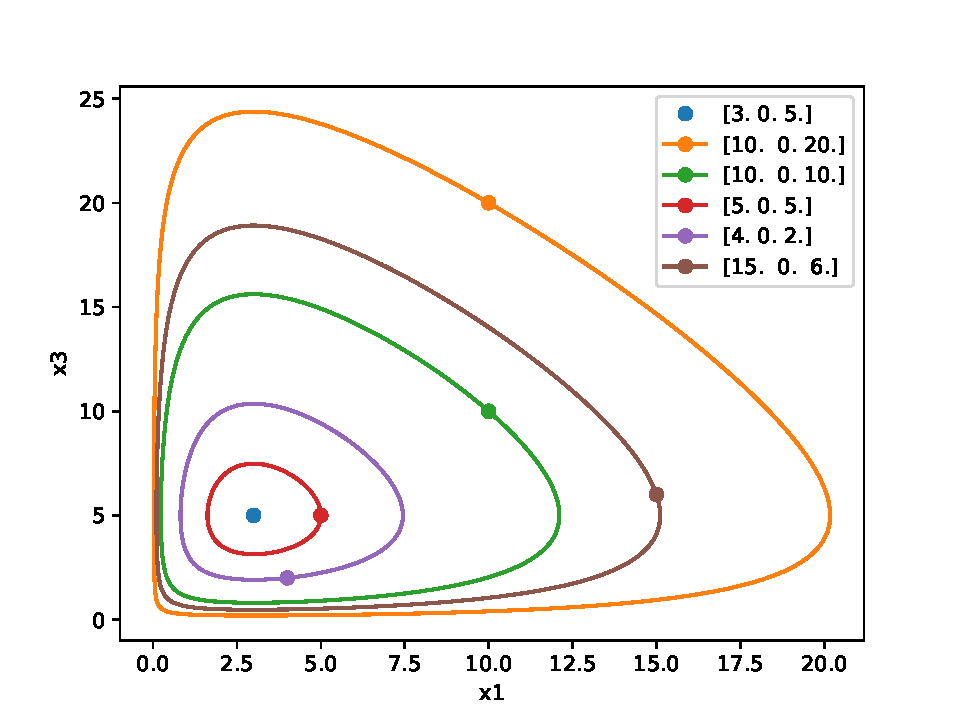
\includegraphics[width=8cm]{pictures/x2_0phase.pdf}
        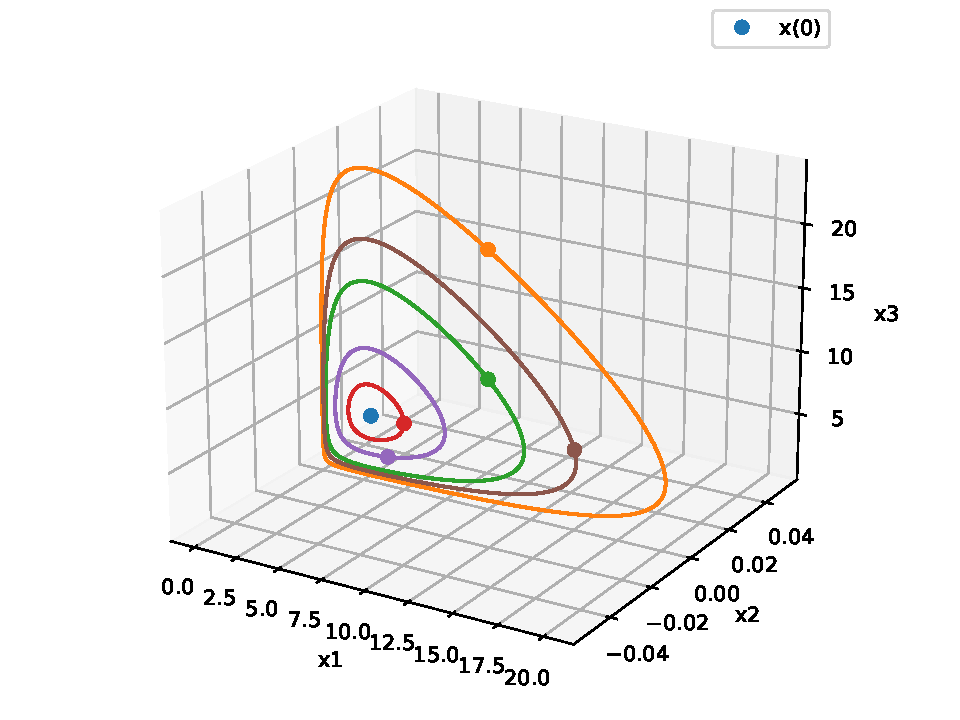
\includegraphics[width=8cm]{pictures/x2_0phase3.pdf}
        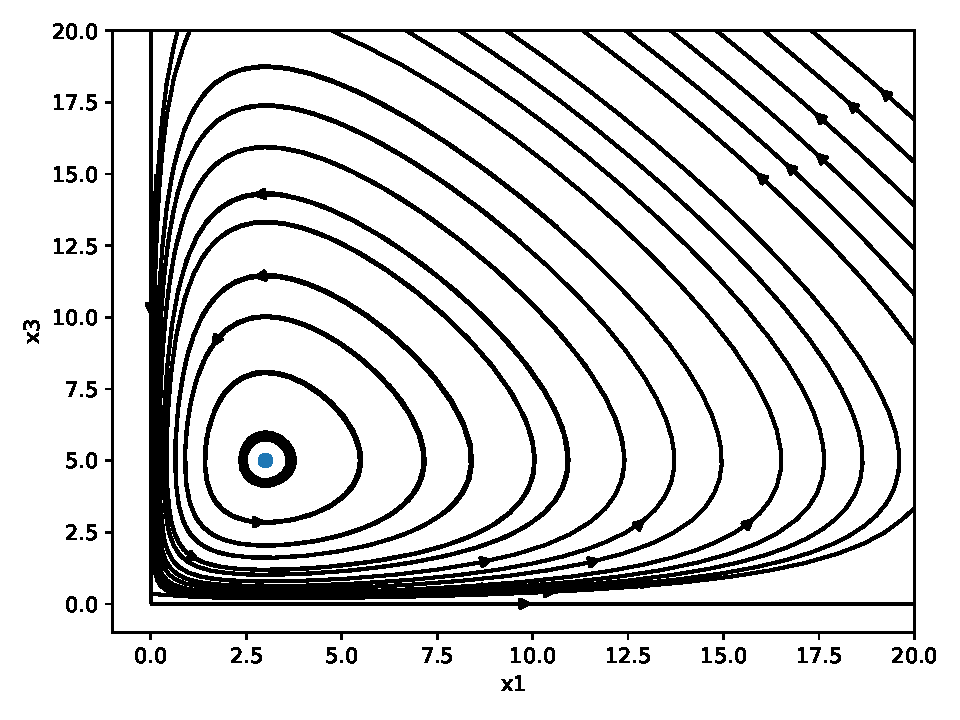
\includegraphics[width=8cm]{pictures/x2_0vector.pdf}
        \caption{На отрезке времени \( [0, 3] \).}
    \end{figure}


    \subsubsection{При вымершей третьей популяции}

    \begin{figure}[H]
        \centering
        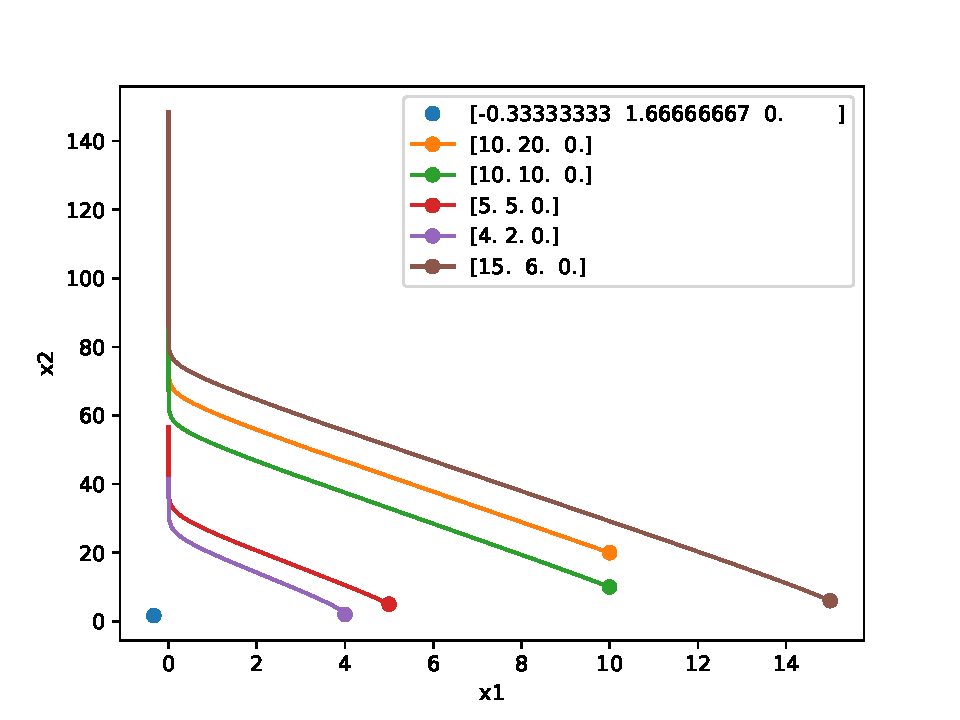
\includegraphics[width=8cm]{pictures/x3_0phase.pdf}
        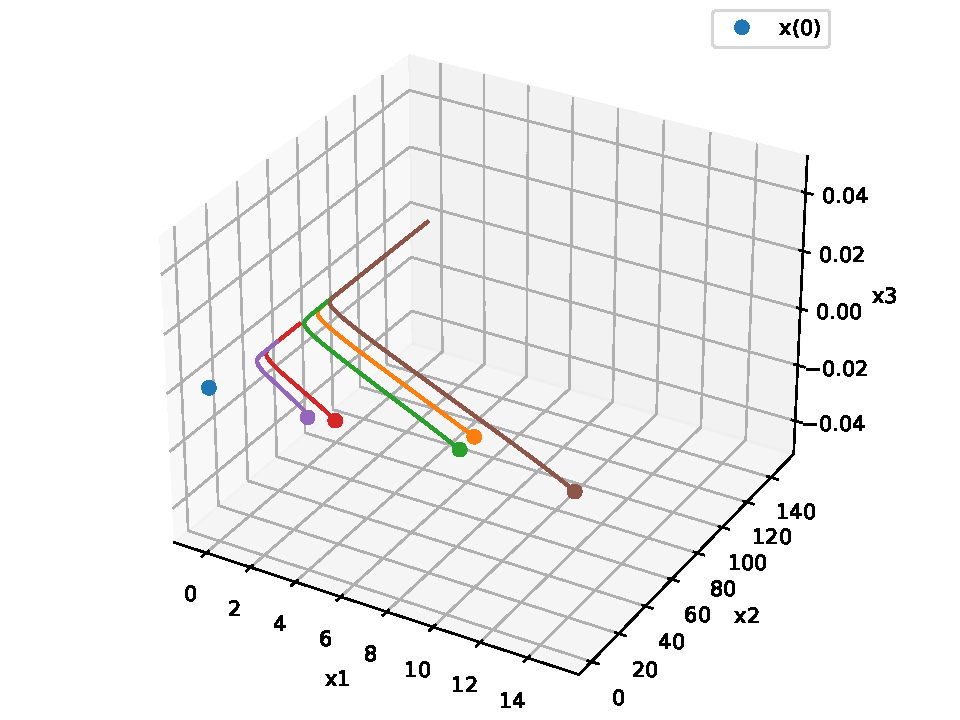
\includegraphics[width=8cm]{pictures/x3_0phase3.pdf}
        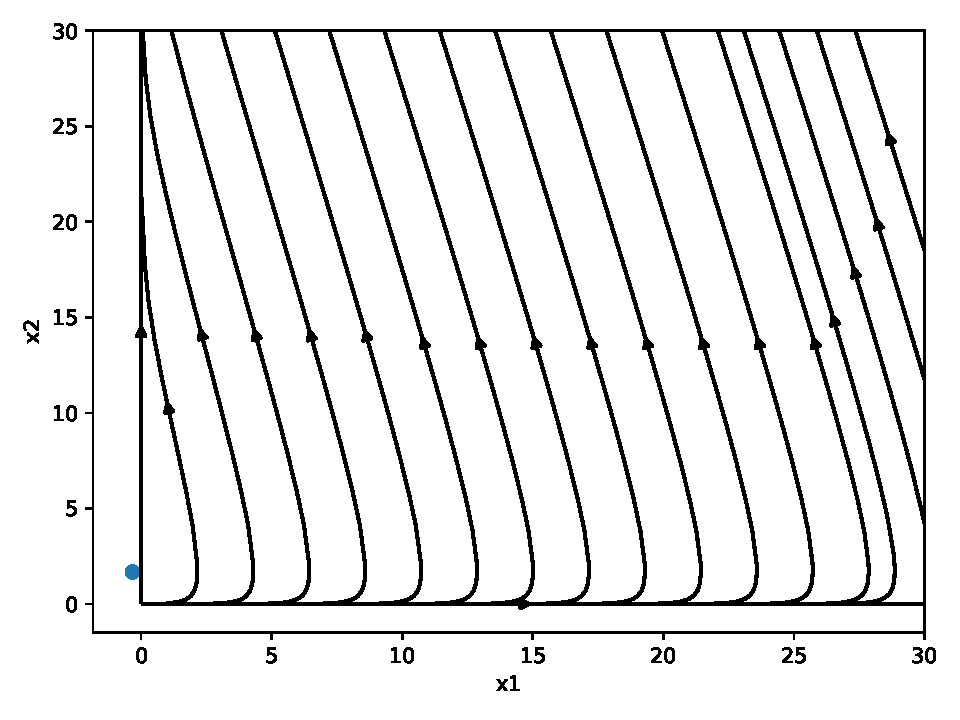
\includegraphics[width=8cm]{pictures/x3_0vector.pdf}
        \caption{На отрезке времени \( [0, 0.1] \).}
    \end{figure}

    \subsubsection{Несколько изначально не вымерших популяций}
    \begin{figure}[H]
        \centering
        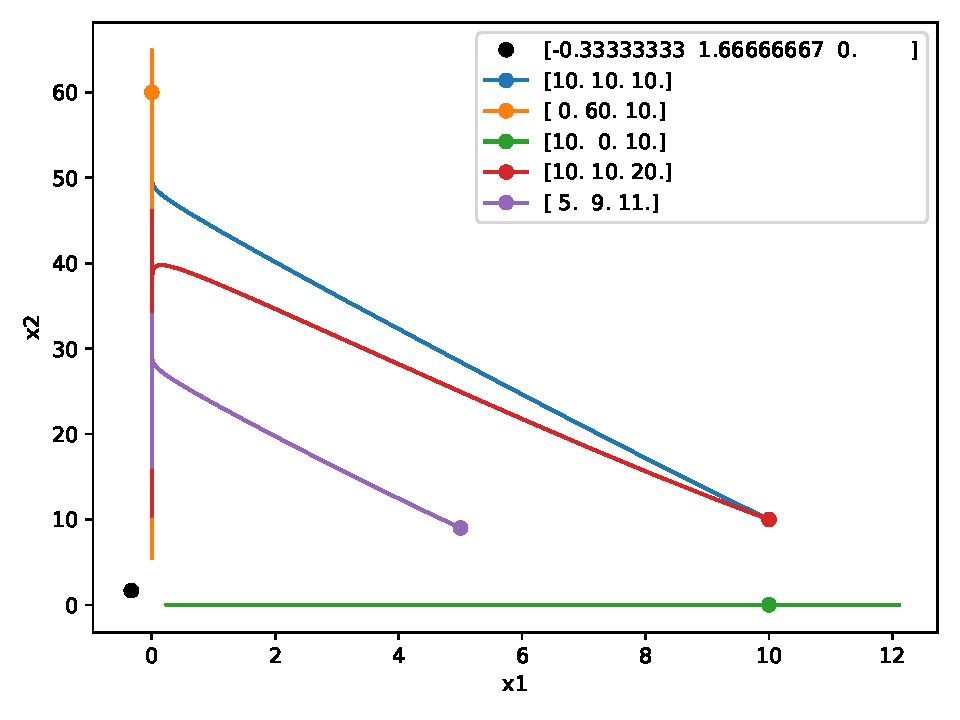
\includegraphics[width=8cm]{pictures/x_12phase.pdf}
        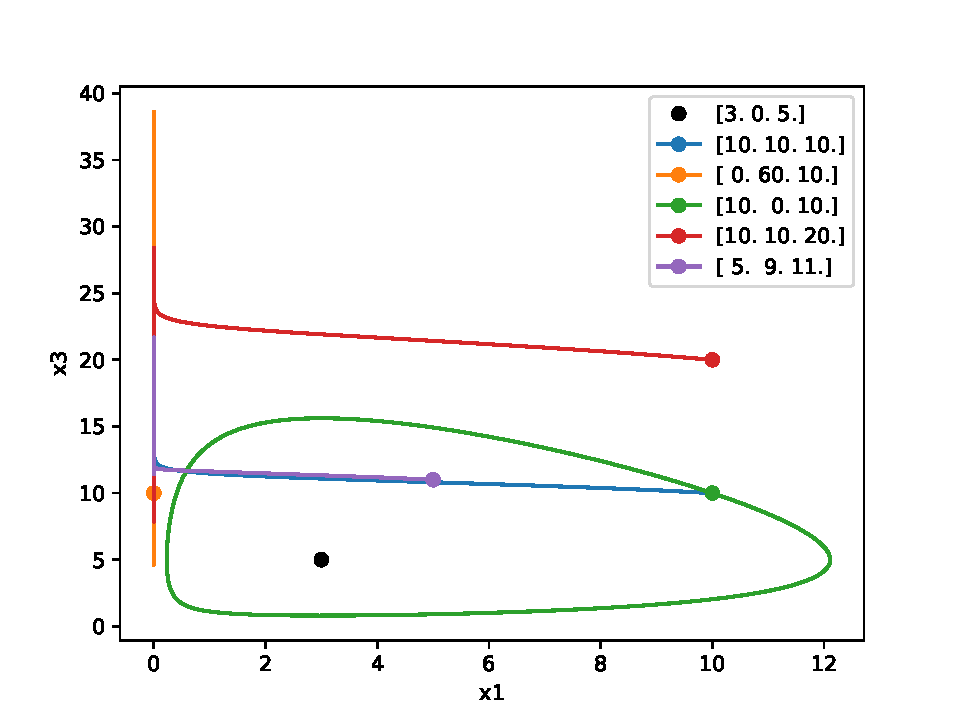
\includegraphics[width=8cm]{pictures/x_13phase.pdf}
        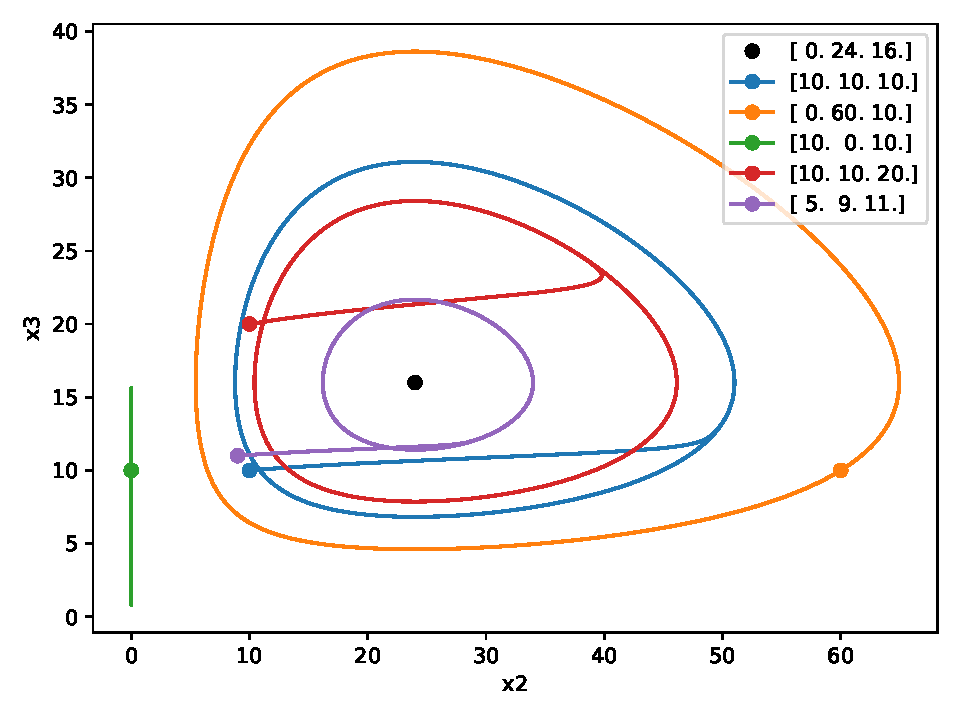
\includegraphics[width=8cm]{pictures/x_23phase.pdf}
        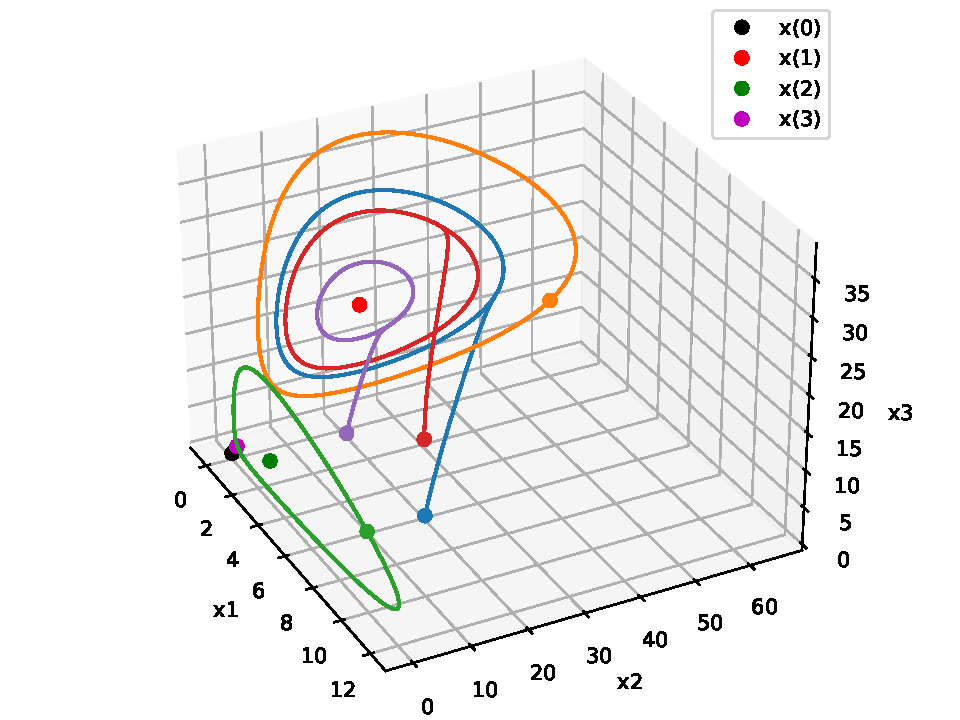
\includegraphics[width=8cm]{pictures/x_phase3.pdf}
        \caption{На отрезке времени \( [0, 3] \).}
    \end{figure}

    \pagebreak
    \subsection{Модель Колмогорова}
    Возьмём такие функции для построения модели:
    \[
        \begin{split}
            & \varepsilon (x_1) = -x_1 + 10, \\
            & K_{12} (x_1) = x_1 - 5, ~ K_{13} (x_1) = x_1 - 3, ~ K_{23} (x_2) = x_2 - 4, \\
            & V_{12} (x_1) = 2 x_1, ~ V_{13} (x_1) = 3 x_1, ~ V_{23} (x_2) = x_2.
        \end{split}
    \]

    \subsubsection{При вымершей первой популяции}

    \begin{figure}[H]
        \centering
        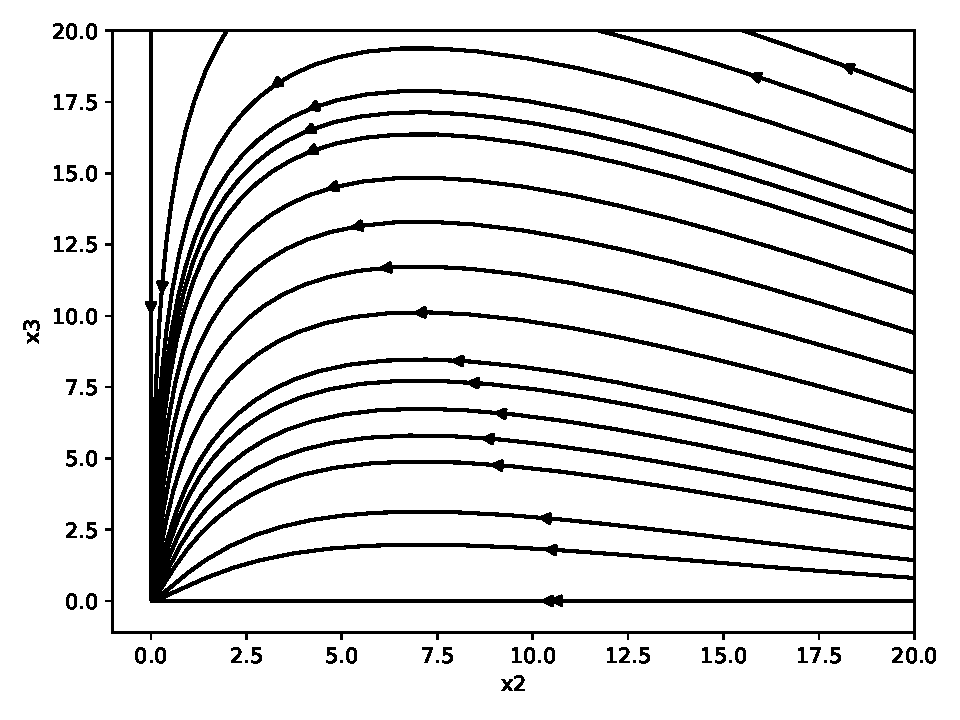
\includegraphics[width=8cm]{pictures/kx1_0vector.pdf}
    \end{figure}


    \subsubsection{При вымершей второй популяции}

    \begin{figure}[H]
        \centering
        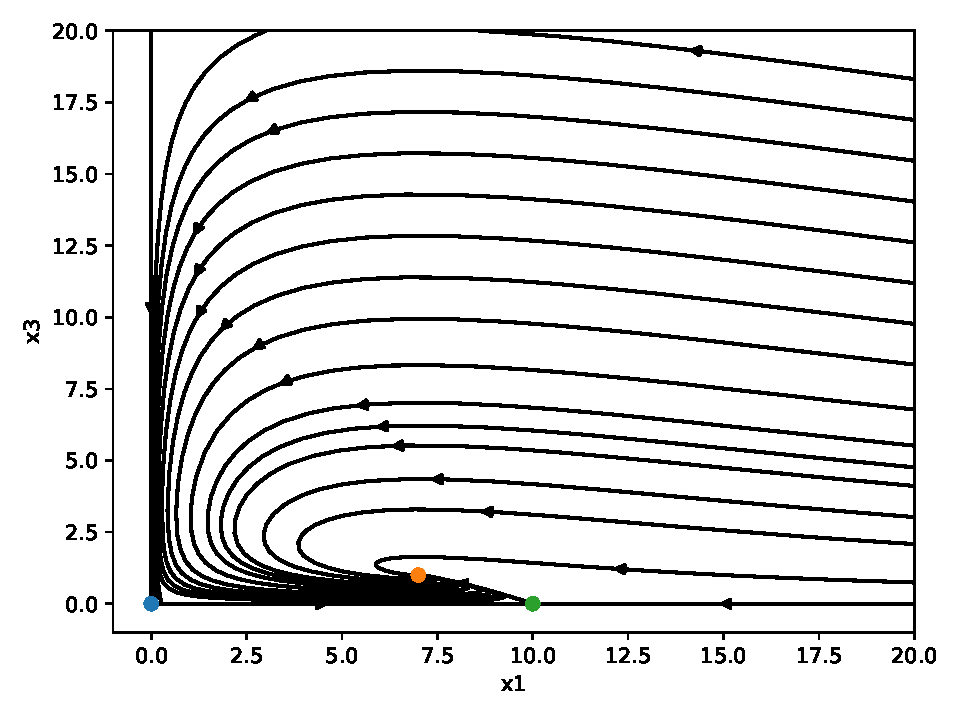
\includegraphics[width=8cm]{pictures/kx2_0vector.pdf}
    \end{figure}


    \subsubsection{При вымершей третьей популяции}

    \begin{figure}[H]
        \centering
        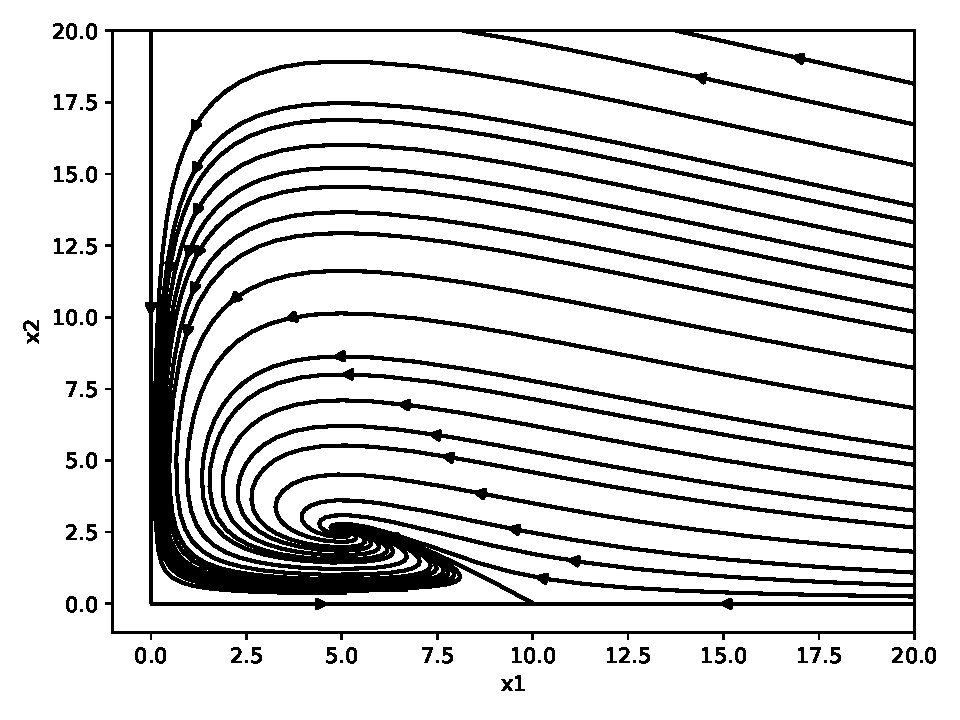
\includegraphics[width=8cm]{pictures/kx3_0vector.pdf}
    \end{figure}

    \subsubsection{Несколько изначально не вымерших популяций}
    \begin{figure}[H]
        \centering
        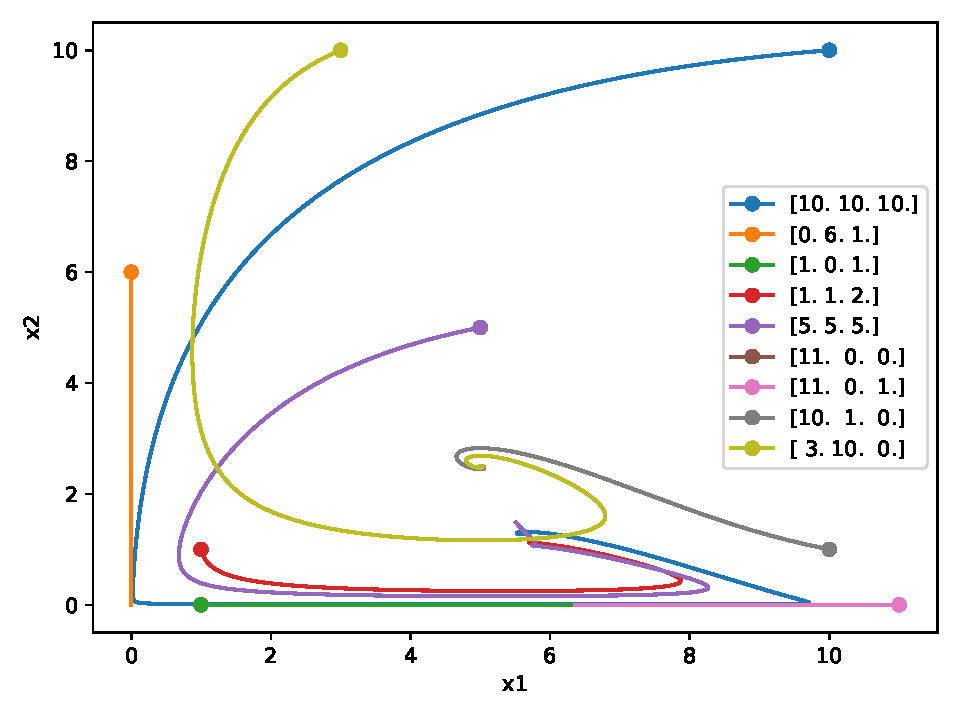
\includegraphics[width=8cm]{pictures/kx_12phase.pdf}
        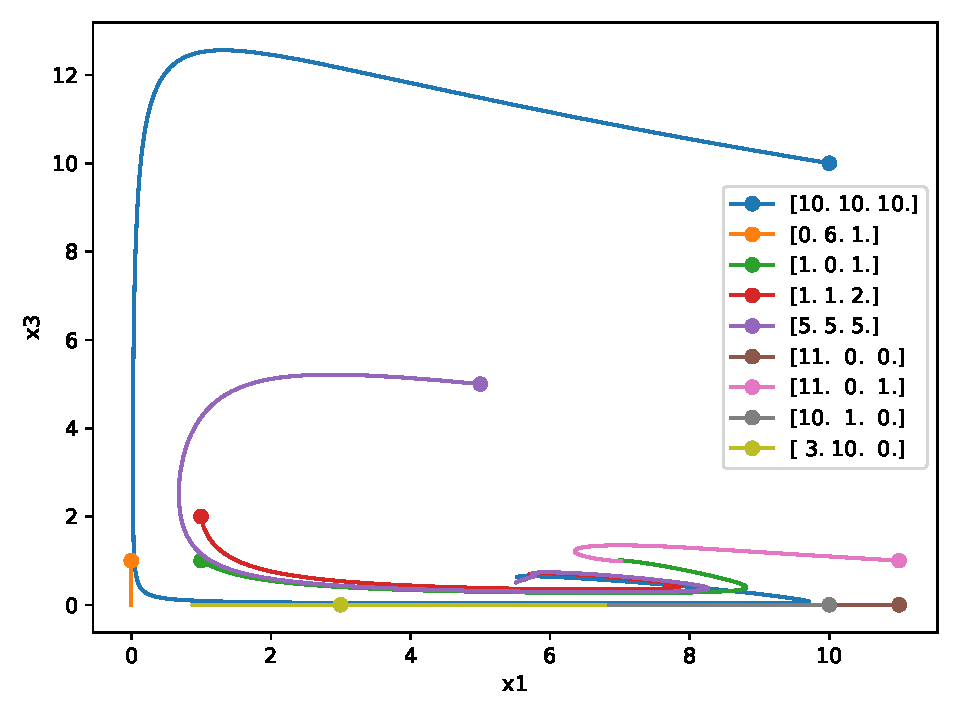
\includegraphics[width=8cm]{pictures/kx_13phase.pdf}
        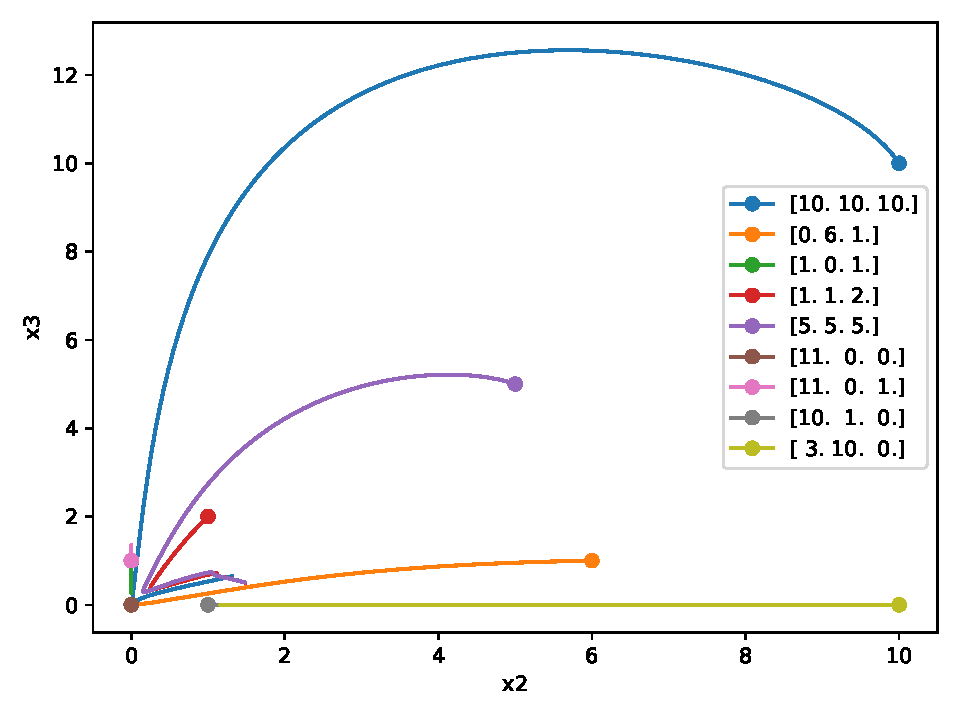
\includegraphics[width=8cm]{pictures/kx_23phase.pdf}
        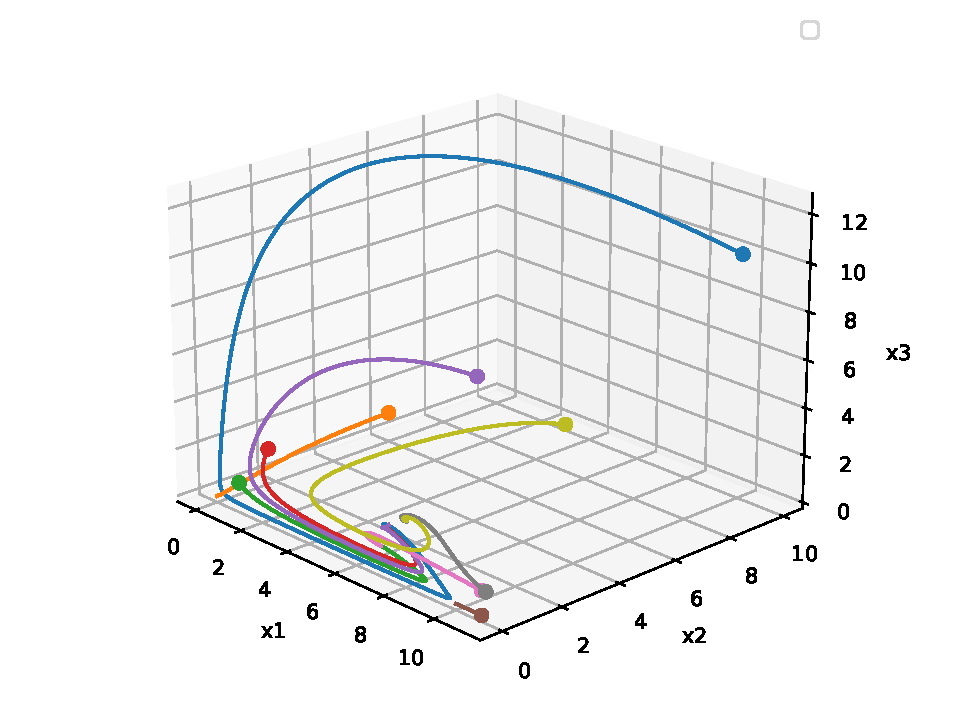
\includegraphics[width=8cm]{pictures/kx_phase3.pdf}
        \caption{На отрезке времени \( [0, 3] \).}
    \end{figure}